\part{Windows Server 2008 R2}
Операционная система \textit{Windows Server 2008 R2}, созданная на основе \textit{Windows Server 2008}, расширяет базовые возможности операционной системы \textit{Windows Server} и предоставляет новые мощные средства, помогая организациям всех размеров повышать управляемость, доступность и гибкость в соответствии с изменяющимися требованиями бизнеса.
Как и \textit{Windows 7}, \textit{Windows Server 2008 R2} использует ядро \textit{Windows NT 6.1}.
Новые возможности включают улучшенную виртуализацию, новую версию \textit{Active Directory}, \textit{Internet Information Services 7.5} и поддержку до 256 процессоров. Система доступна только в 64-разрядном варианте.

\section{Получение дистрибутива}
Система \textit{Windows Server 2008 R2} является платным серверным решением корпорации \textit{Microsoft}, получить ознакомительный дистрибутив можно на странице \textit{центра пробного програмного обеспечения TechNet}\footnote{http://technet.microsoft.com/ru-ru/evalcenter/} портала \textit{Microsoft TechNet}.

\section{Выбор выпуска}
\textit{Windows Server 2008 R2} поставляется в нескольких редакциях, приведем сравнительную таблицу версий основанную на ролях сервера:
\begin{figure}[H]
\center{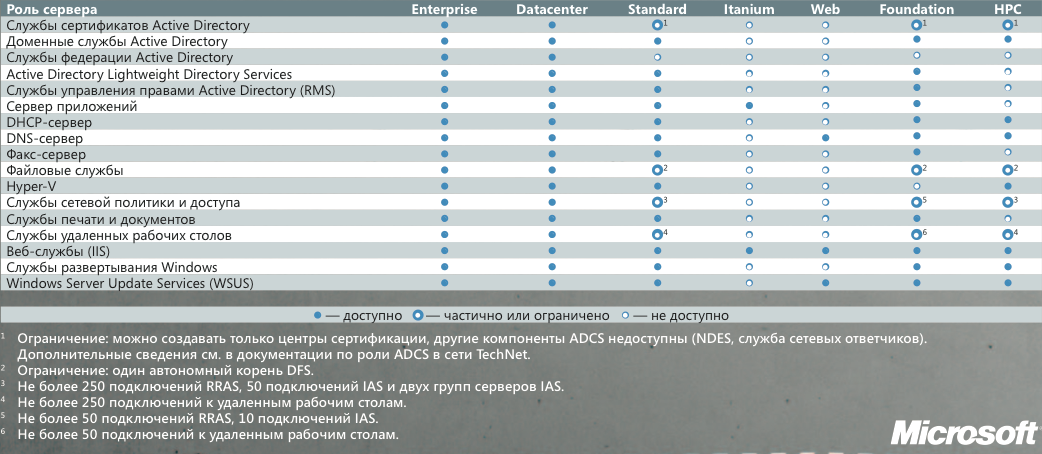
\includegraphics[width=1\linewidth]{ws2k8/diff.png}}
\end{figure}
Как мы видим для наших целей(AD, DNS, DHCP) подойдет выпуск \textit{Standard}.

\section{Установка}
Установка.

\section{Настройка}
Настройка.

\subsection{Шаг 1}
Поднимаем Active Directory.

\subsection{Шаг 2}
Что-нибудь еще\ldots